\section{Geometry of $\mathbb{R}^n$}

Each vector $\begin{bmatrix}v_1\\v_2 \\ \vdots \\ v_n \end{bmatrix} \in \mathbb{R}^n$ can be visualized as an arrow going from the origin 
$(0,0, \ldots, 0)$ to the point $(v_1, v_2, \ldots, v_n)$.  In this case we'd call the \textbf{base point} the origin.

\begin{example}
$\begin{bmatrix}2\\5\end{bmatrix}$ can be visualized as the arrow between $(0,0)$ and $(2,5)$\\
\begin{center}
  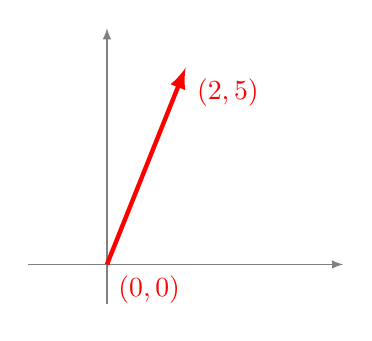
\begin{tikzpicture}[scale=.5]
    \coordinate (Origin)   at (0,0);
    \coordinate (XAxisMin) at (-2,0);
    \coordinate (XAxisMax) at (6,0);
    \coordinate (YAxisMin) at (0,-1);
    \coordinate (YAxisMax) at (0,6);
    \draw [thin, gray,-latex] (XAxisMin) -- (XAxisMax);% Draw x axis
    \draw [thin, gray,-latex] (YAxisMin) -- (YAxisMax);% Draw y axis
    \draw [ultra thick,-latex,red] (Origin) node [below right] {$(0,0)$} -- (2,5) node [below right] {$(2,5)$};
  \end{tikzpicture}
\end{center}
\end{example}

We can also think of any arrow from point $(a_1, a_2, \ldots, a_n)$ to point $(b_1, b_2, \ldots, b_n)$ as a vector. We've simply changed 
the \text{base point} to $(a_1, a_2, \ldots, a_n)$ instead of the origin. 

\begin{definition}
The \textbf{canonical form} of a vector from $(a_1, a_2, \ldots, a_n)$ to $(b_1, b_2, \ldots, b_n)$ is the vector 
$\begin{bmatrix}b_1-a_1 \\ b_2-a_2 \\ \vdots \\ b_n-a_n\end{bmatrix}$
\end{definition}

\begin{remark}
You can think of the canonical form of a vector is taking an arrow with the same length and direction with base point of the origin.
\end{remark}

\begin{example}
The vector from $(2,3)$ to $(3,-2)$ has canonical form $\begin{bmatrix*}[C]1\\-5\end{bmatrix*}$. Below the vector is in red and the canonical form of the vector is in blue.\\
\begin{center}
  \begin{tikzpicture}[scale=.5]
    \coordinate (Origin)   at (0,0);
    \coordinate (XAxisMin) at (-6,0);
    \coordinate (XAxisMax) at (6,0);
    \coordinate (YAxisMin) at (0,-6);
    \coordinate (YAxisMax) at (0,6);
    \draw [thin, gray,-latex] (XAxisMin) -- (XAxisMax);% Draw x axis                                                                                                   
    \draw [thin, gray,-latex] (YAxisMin) -- (YAxisMax);% Draw y axis                                                                                                   
    \draw [ultra thick,-latex,red] (2,3) node [above right] {$(2,3)$} -- (3,-2) node [above right] {$(3,-2)$};
    \draw [ultra thick,-latex,blue] (Origin) node [above right] {$(0,0)$} -- (1,-5) node [above right] {$(3,-2)$};
  \end{tikzpicture}
  \end{center}
\end{example}

\subsection{Scalar Multiplication and Vector Addition}

Scalar multiplication can be thought of as a  geometric operation. If $r>0$ then $r\vec{v}$ can be thought of as $v$ stretched or shrunk by real factor $r$.\\ 
\begin{center}
\begin{tikzpicture}[scale=.5]
    \coordinate (Origin)   at (0,0);
    \coordinate (XAxisMin) at (-6,0);
    \coordinate (XAxisMax) at (6,0);
    \coordinate (YAxisMin) at (0,-6);
    \coordinate (YAxisMax) at (0,6);
    \draw [thin, gray,-latex] (XAxisMin) -- (XAxisMax);% Draw x axis                                                                                                   
    \draw [thin, gray,-latex] (YAxisMin) -- (YAxisMax);% Draw y axis                                                                                                   
    \draw [ultra thick,-latex,blue] (0,0)  -- (6,3) node[pos=0.5,above]{$r\vec{v}$};
    \draw [ultra thick,-latex,black] (Origin) -- (2,1) node[pos=0.5,above]{$\vec{v}$};;
\end{tikzpicture}
\end{center}
If $r<0$ then $r\vec{v}$ can be thought of as $v$ reflected through the origin then stretced or shrunk by a real factor $|r|$
\begin{center}
\begin{tikzpicture}[scale=.5]
    \coordinate (Origin)   at (0,0);
    \coordinate (XAxisMin) at (-6,0);
    \coordinate (XAxisMax) at (6,0);
    \coordinate (YAxisMin) at (0,-6);
    \coordinate (YAxisMax) at (0,6);
    \draw [thin, gray,-latex] (XAxisMin) -- (XAxisMax);% Draw x axis                                                                                                   
    \draw [thin, gray,-latex] (YAxisMin) -- (YAxisMax);% Draw y axis                                                                                                   
    \draw [ultra thick,-latex,blue] (0,0)  -- (-6,-3) node[pos=0.5,above]{$r\vec{v}$};
    \draw [ultra thick,-latex,black] (Origin) -- (2,1) node[pos=0.5,above]{$\vec{v}$};;
\end{tikzpicture}
\end{center}
Vector addition can also be thought of as a geometric operation via the \textbf{parallelogram rule}. 

\begin{proposition}[The Paralelogram Rule] If $\vec{v},\vec{w} \in \mathbb{R}^n$ with then $\vec{v}+\vec{w}$ can be determined by the following:
\begin{enumerate}
\item If there is a nonzero linear combination $s\vec{v}+t\vec{w}$ equal to $\vec{0}$ then 
$\vec{v}+\vec{w}$ is either a scalar multiple of $\vec{v}$ or a scalar multiple of $\vec{w}$.

\item Otherwise $\vec{v}+\vec{w}$ is determined by the parallelogram rule:\\
\begin{center}
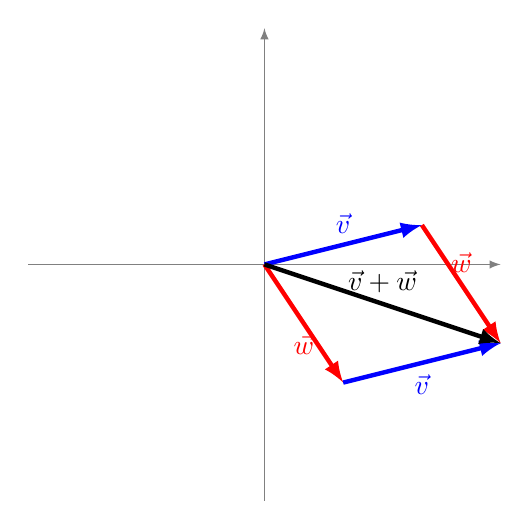
\begin{tikzpicture}[scale=.5]
    \coordinate (Origin)   at (0,0);
    \coordinate (XAxisMin) at (-6,0);
    \coordinate (XAxisMax) at (6,0);
    \coordinate (YAxisMin) at (0,-6);
    \coordinate (YAxisMax) at (0,6);
    \draw [thin, gray,-latex] (XAxisMin) -- (XAxisMax);% Draw x axis                                                                                                   
    \draw [thin, gray,-latex] (YAxisMin) -- (YAxisMax);% Draw y axis                                                                                                   
    \draw [ultra thick,-latex,blue] (0,0)  -- (4,1) node[pos=0.5,above]{$\vec{v}$};
    \draw [ultra thick,-latex,red] (4,1)  -- (6,-2) node[pos=0.5,above]{$\vec{w}$};
    \draw [ultra thick,-latex,red] (Origin) -- (2,-3) node[pos=0.5,below]{$\vec{w}$};;
    \draw [ultra thick,-latex,blue] (2,-3)  -- (6,-2) node[pos=0.5,below]{$\vec{v}$};
    \draw [ultra thick,-latex,black] (0,0)  -- (6,-2) node[pos=0.5,above]{$\vec{v}+\vec{w}$};
\end{tikzpicture}
\end{center}
Note that taking the base point of $\vec{w}$ to be the end point of $\vec{v}$ yeilds the same result as taking the base point of $\vec{v}$ to be the end point of 
$\vec{w}$.
\end{enumerate}
\end{proposition}
\begin{proof}
The proof of the case where there is a nonzero linear combination of $s\vec{v}+t\vec{w}=\vec{0}$ is Exercise~\ref{exercise:dependent_addition}. This case eliminates the possiblity that $\vec{v}$ and $\vec{w}$ are on the same line.

The vector $\vec{v}$ take the origin $(0,0, \ldots, 0)$ to the coordinate $(v_1, v_2, \ldots, v_n)$. 
By adding vector $w$ we take $(v_1, v_2, \ldots, v_n)$ to $(v_1+w_1, v_2+w_2, \ldots, v_n+w_n)$. 
So $v+w$ is the composite operation of taking the origin to $(v_1, v_2, \ldots, v_n)$ then to $(v_1+w_1, v_2+w_2, \ldots, v_n+w_n)$. 

Graphically we can think of this as follow the canonical form of $\vec{v}$ then base $w$ at the endpoint of $v$ to get $\vec{v}+\vec{w}$. Since we can do the same thing starting with $w$, this makes a parallelogram as long as $\vec{v}$ and $\vec{w}$ are not on the same line.
\end{proof}

\begin{example} 
Let $\vec{v}=\begin{bmatrix} 1 \\ 3 \end{bmatrix}$ and $\vec{w}=\begin{bmatrix*}[C] -5 \\ 2 \end{bmatrix*}$. We can identify all vectors in $\mathbb{R}^n$ as a linear combination of these two geometrically. Since the canonical forms of$\vec{v}$ and $\vec{w}$ are not in the same line in $\mathbb{R}^n$, $\vec{v}+\vec{w}$ forms a parallelogram. Below we mark all the integer linear combination endpoints of $m\vec{v}+n\vec{w}$ where $n$ and $m$ are integers. This makes a shape called a lattice:
\begin{center}
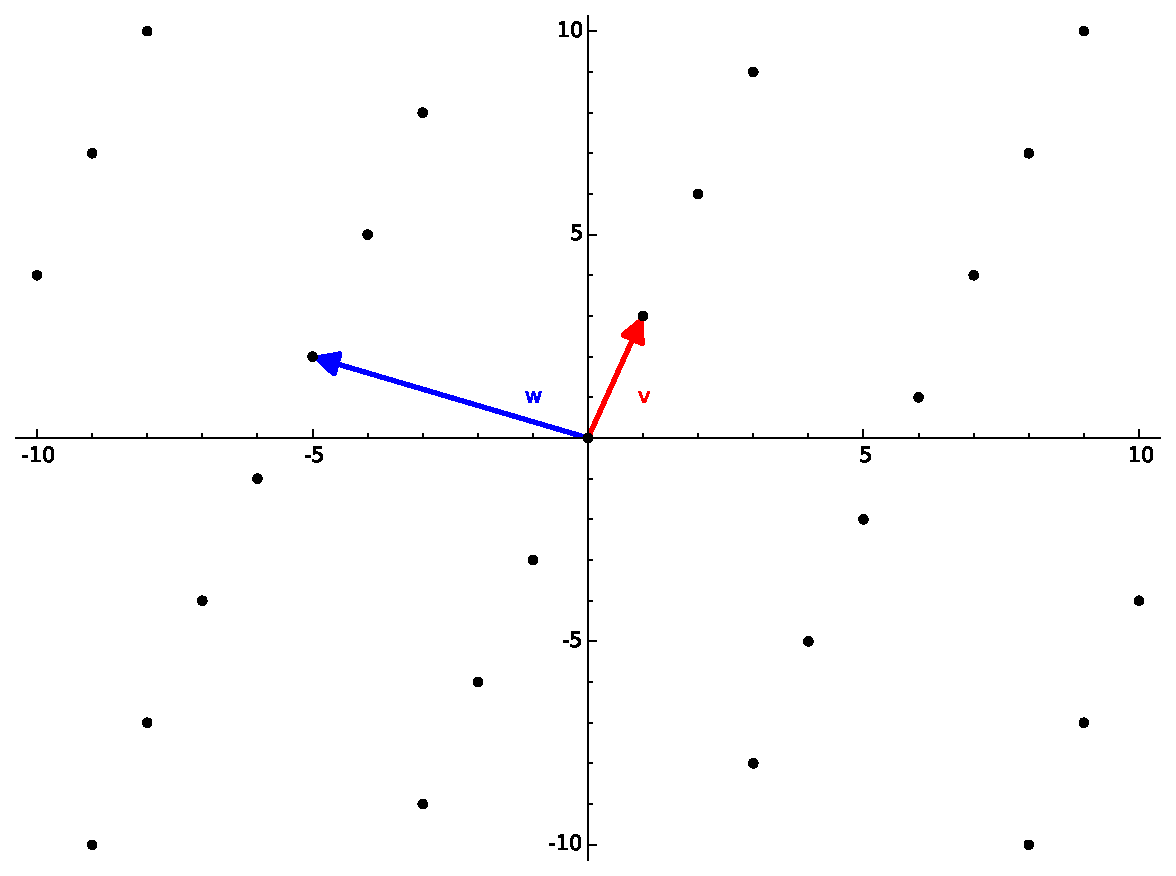
\includegraphics[scale=.5]{Rn/vw_graph1.pdf}
\end{center}

We can see below that the vector $\begin{bmatrix*}[C]9 \\ -7 \end{bmatrix*}$ can be written by the linear combination $(-1)\vec{v}+(-2)\vec{w}$. It doesn't even mater what path we use to get there since we can use the associative properties of vector addition and the distributive property of vector addition and scalar multiplication.
\begin{center}
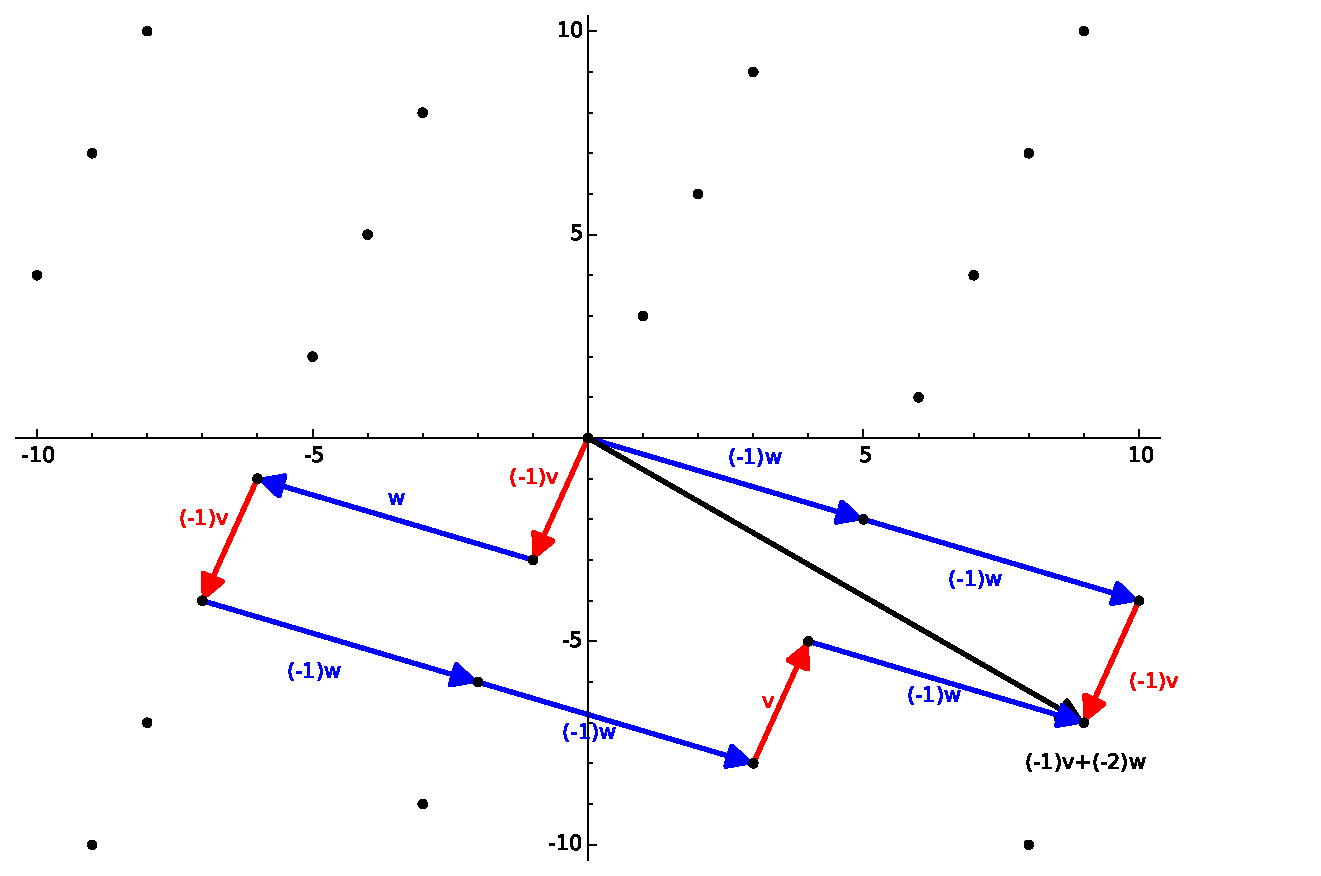
\includegraphics[scale=.5]{Rn/vw_9n7_graph1.pdf}
\end{center}

It's not a very large stretch to include vectors with endpoints on the rest of the plane since all we need to allow is any real linear combination $r\vec{v}+t\vec{w}$ where $r$ and $t$ are real numbers. For instance we can add in the endpoint $(3,3)$ by taking $\frac{21}{17}\vec{v}+\frac{-6}{17}\vec{w}$\\
\begin{center}
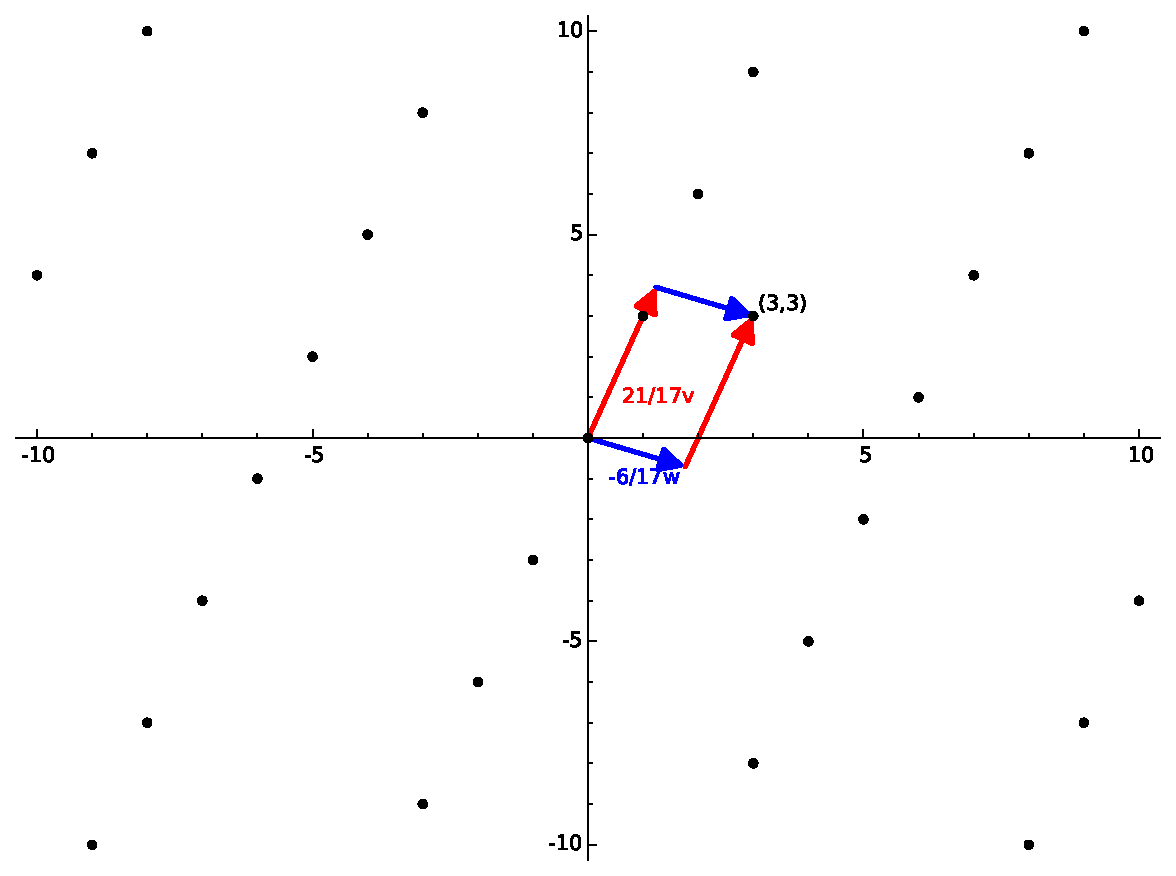
\includegraphics[scale=.5]{Rn/vw_graph2.pdf}\
\end{center}
\end{example}
\begin{remark}
The above example illustrates that you can build a whole plane with linear combinations of two vectors.
\end{remark}
\begin{definition}[The Span]
We call the set of linear combinations of a collection of vectors in $\mathbb{R}^n$ the \textbf{span}.
\[
\text{span}\{ \vec{v}_1, \vec{v}_2, \ldots, \vec{v}_k \}=
\{a_1\vec{v}_1+a_2\vec{v}_2+\cdots+a_k\vec{v}_k \mid a_1, a_2, \ldots , a_k \in \mathbb{R} \}
\]
\end{definition}

\begin{example} Consider the following span
\[
H=\text{span}\left\{
\begin{bmatrix*}[C]1 \\ 0 \\ 0 \\ -1\end{bmatrix*},
\begin{bmatrix*}[C]-1 \\ 2 \\ 1 \\ 0\end{bmatrix*},
\begin{bmatrix*}[C]0 \\ 1 \\ 1 \\ 1\end{bmatrix*}
\right\}
\]

Each $\vec{v} \in H$ can be written as a liner combination:
\[
\vec{v}=
x_1\begin{bmatrix*}[C]1 \\ 0 \\ 0 \\ -1\end{bmatrix*}+
x_2\begin{bmatrix*}[C]-1 \\ 2 \\ 1 \\ 0\end{bmatrix*}+
x_3\begin{bmatrix*}[C]0 \\ 1 \\ 1 \\ 1\end{bmatrix*}
\]
for some choice of $x_1, x_2, x_3 \in \mathbb{R}$. This in turn can be written
as matrix vector multiplication:
\[
\vec{v}=
x_1\begin{bmatrix*}[C]1 \\ 0 \\ 0 \\ -1\end{bmatrix*}+
x_2\begin{bmatrix*}[C]-1 \\ 2 \\ 1 \\ 0\end{bmatrix*}+
x_3\begin{bmatrix*}[C]0 \\ 1 \\ 1 \\ 1\end{bmatrix*}
=
\begin{bmatrix*}[C]
1 & -1 & 0 \\
0 & 2 & 1 \\
0 & 1 & 1 \\
-1 & 0 & 1 
\end{bmatrix*}
\begin{bmatrix}
x_1 \\ x_2 \\ x_3
\end{bmatrix}
\]

So the linear transformation $T:\mathbb{R}^3 \to \mathbb{R}^4$ defined by 
\[
T(\vec{x})=\begin{bmatrix*}[C]
1 & -1 & 0 \\
0 & 2 & 1 \\
0 & 1 & 1 \\
-1 & 0 & 1 
\end{bmatrix*}
\begin{bmatrix}x_1 \\ x_2 \\ x_3 \end{bmatrix}
\]
takes coordinates on each of the vectors to the appropriate linear combination in $H$.
\end{example}
\begin{example} We can describe the image of a linear transformation using a span quite easily. For example $T:\mathbb{R}^3 \to \mathbb{R}^5$ defined by
\[
T(\vec{v})=\begin{bmatrix*}[C]
1 & 0 & -1 \\
0 & -1 & 5 \\
2 & 0 & 0 \\
-3 & 3 & 3 \\
3 & 3 & -2 \\
\end{bmatrix*}\begin{bmatrix}v_1\\ v_2\\ v_3\end{bmatrix}
=
v_ 1\begin{bmatrix*}[C]1 \\ 0 \\ 2 \\ -3 \\ 3 \end{bmatrix*}
+v_2\begin{bmatrix*}[C]0 \\ -1 \\ 0 \\ 3 \\ 3 \end{bmatrix*}
+v_3\begin{bmatrix*}[C]-1 \\ 5 \\ 0 \\ 3 \\ 2 \end{bmatrix*}
\] 

So we can rewrite the image of $T$ as 

\[
\text{span}\left\{
\begin{bmatrix*}[C]1 \\ 0 \\ 2 \\ -3 \\ 3 \end{bmatrix*},
\begin{bmatrix*}[C]0 \\ -1 \\ 0 \\ 3 \\ 3 \end{bmatrix*},
\begin{bmatrix*}[C]-1 \\ 5 \\ 0 \\ 3 \\ 2 \end{bmatrix*}
\right\}
=\left\{
v_ 1\begin{bmatrix*}[C]1 \\ 0 \\ 2 \\ -3 \\ 3 \end{bmatrix*}
+v_2\begin{bmatrix*}[C]0 \\ -1 \\ 0 \\ 3 \\ 3 \end{bmatrix*}
+v_3\begin{bmatrix*}[C]-1 \\ 5 \\ 0 \\ 3 \\ 2 \end{bmatrix*}
\mid 
v_1, v_2, v_3 \in \mathbb{R}^5 
\right\}
\]
\end{example}
\subsubsection{Exercises}

\begin{exercise} Find the canonical form of each of the following vectors:\\
\begin{inparaenum}[a)]
\item a vector from $(0,0)$ to $(1,3)$ in $\mathbb{R}^2$\\
\item a vector from $(1,2)$ to $(5,6)$ in $\mathbb{R}^2$\\
\item a vector from $(0,0,1)$ to $(-3,1,5)$ in $\mathbb{R}^3$\\
\item a vector from $(3,0,-2)$ to $(0,0,0)$ in $\mathbb{R}^3$\\
\end{inparaenum}
\end{exercise}

\begin{exercise} Draw a lattice of enpoints of vectors $\vec{u}=\begin{bmatrix}2\\1\end{bmatrix}$ and $\vec{v}=\begin{bmatrix}1\\-5\end{bmatrix}$. That is graph 
$m\vec{u}+n\vec{v}$ for integer values of $m$ and $n$. Use the lattice to graphically determine, or estimate, the coefficients $r$ and $t$ for the linear combination of $r\vec{u}+t\vec{v}$ that gives the vector below:\\
\begin{inparaenum}
\item $\begin{bmatrix}3 \\ 7 \end{bmatrix}$\hfill 
\item $\begin{bmatrix*}[C]-1 \\ -6 \end{bmatrix*}$\hfill {} \\
\item $\begin{bmatrix*}[C]-9 \\ 1 \end{bmatrix*}$\hfill 
\item $\begin{bmatrix*}[C] 0 \\ -5.5 \end{bmatrix*}$\hfill {} \\
\end{inparaenum}
\end{exercise}



\subsection{Linear Dependence and Linear Independence}

Previously, we noticed that when we add two vectors $\vec{v}+\vec{w}$, the result can geometrically be described either by linear addition or by the parallelogram rule. When the result is linear addition the vectors are on the same line in $\mathbb{R}^n$. In other words $\vec{v}=r\vec{w}$ or $\vec{w}=t\vec{v}$ for some $r,t \in \mathbb{R}$. Instead of stating this as two cases, we can instead write 

\begin{equation*}
a\vec{v}+b\vec{w}=\vec{0}
\end{equation*}

where $a$ and $b$ are real scalars and they are not both zero. We call the case where both $a=0$ and $b=0$ the \textbf{trivial solution} to the vector equation and any solution where at least one of them is non-zero a \textbf{non-trivial solution}.

Generalizing to more than two vectors we get the following definition:

\begin{definition}[Linearly Dependent Vectors]
Vectors $\vec{v}_1, \vec{v}_2, \ldots, \vec{v}_n \in \mathbb{R}^m$ are \textbf{linearly dependent} if 

$$x_1\vec{v}_1+x_2\vec{v}_2+\cdots + x_n \vec{v}_n=\vec{0}$$

has a \textbf{non-trivial solution}. That is, there is a solution $x_1, x_2, \ldots, x_n$ to the vector equation with $x_i \neq 0$ for at least one value $i$. 
\end{definition}
\begin{proposition} Vectors $\vec{v}$ and $\vec{w}$ in $\mathbb{R}^n$ are linearly dependent if and only if either $\vec{v}=\alpha \vec{w}$ or $\vec{w}=\alpha\vec{v}$ for some real number $\alpha$
\end{proposition}
\begin{proof}
Let $\vec{v}$ and $\vec{w}$ be linearly dependent then there is a nontrivial linear combination:
\[
r\vec{v}+t\vec{w}=\vec{0}
\]
where one of $r$ or $t$ is not zero. If $r \neq 0$ then $\vec{v}=-\frac{t}{r}\vec{w}$ and $\alpha=-\frac{t}{r}$. If $t \neq 0$ then $\vec{w}=-\frac{r}{t}\vec{v}$ and $\alpha=-\frac{r}{t}$.

Let $\vec{v}=\alpha \vec{w}$ then $\vec{0}=(-1)\vec{v}+\alpha\vec{w}$ is a nontrivial linear combination since $-1 \neq 0$. 
%
Let $\vec{w}=\alpha\vec{v}$ then $\vec{0}=(-1)\vec{w}+\alpha\vec{v}$ is a nontrivial linear combination since $-1 \neq 0$. 
\end{proof}

\begin{proposition} Vectors $\vec{v}_1, \vec{v}_2, \ldots, \vec{v}_n \in \mathbb{R}^n$ are linearly dependent if and only if at at least one of the vectors, $\vec{v}_k$, can be written as a linear combination of the others. That is,
$$
\vec{v}_k=\alpha_1 v_1+ \cdots+ \alpha_{k-1}\vec{v}_{k-1}+ \alpha_{k+1}\vec{v}_{k+1}+\cdots+ \alpha_n \vec{v}_n
$$
\end{proposition}
\begin{proof}
Let $\vec{v}_1, \vec{v}_2, \ldots, \vec{v}_n \in \mathbb{R}^n$ be linearly dependent. Then there is a nontrivial solution to:

$$x_1\vec{v}_1+x_2\vec{v}_2+\cdots +x_{k-1}\vec{v}_{k-1}+ x_k\vec{v}_k+x_{k+1}\vec{v}_{k+1}+ \cdots + x_n \vec{v}_n=\vec{0}$$

That is $x_k \neq 0$ for some $k$. Solving for $x_k\vec{v}_k$ we get

$$
(-x_k)\vec{v}_k=x_1 v_1+ \cdots + x_{k-1}\vec{v}_{k-1}+ x_{k+1}\vec{v}_{k+1}+\cdots+ x_n \vec{v}_n
$$

Since $x_k \neq 0$ we can multiply both sides of the equation by $-\frac{1}{x_k}$ yeilding:

$$
\vec{v}_k=\frac{x_1}{-x_k} v_1+ \cdots + \frac{x_{k-1}}{-x_k}\vec{v}_{k-1}+ \frac{x_{k+1}}{-x_k}\vec{v}_{k+1}+\cdots+ \frac{x_n}{-x_k} \vec{v}_n
$$

To show the converse let 

$$\vec{v}_k=\alpha_1 v_1+ \cdots+ \alpha_{k-1}\vec{v}_{k-1}+ \alpha_{k+1}\vec{v}_{k+1}+\cdots+ \alpha_n \vec{v}_n$$

Then by adding $(-1)\vec{v}_k$ to both sides
$$
\vec{0}=\alpha_1 v_1+ \cdots+ \alpha_{k-1}\vec{v}_{k-1}+(-1)\vec{v}_k+ \alpha_{k+1}\vec{v}_{k+1}+\cdots+ \alpha_n \vec{v}_n
$$

This is a non-trivial linear combination of $\vec{v}_1, \vec{v}_2, \ldots, \vec{v}_k$ since the $k$-coefficient $(-1)$ is nonzero. Therefore, $\vec{v}_1, \vec{v}_2, \ldots, \vec{v}_k$ are linearly dependent.
\end{proof}

\begin{remark}
The above proposition shows that a linearly dependent set has ``extra vectors'' when it comes to making linear combinations. That is, by adding in a vector $\vec{v}_k$, that can be written as a linear combination of the others you could have accomplished the same thing by simply changing the coefficients on the other vectors. So in a sense the $\vec{v}_k$ vector is unnecessary or ``extra'' and there could be more than one such vector.
\end{remark}

\begin{proposition}\label{prop:zero_dependent} If the zero vector is in a set of vectors then the set is linearly dependent. 
\end{proposition}
\begin{proof}
Left as an exercise.
\end{proof}


\begin{proposition}\label{prop:not_onto} If the row vectors of matrix $A \in M_{m\times n}(\mathbb{R})$ are linearly dependent, then there is a  $\vec{b} \in \mathbb{R}^m$ such that $A\vec{v}=\vec{b}$ does not have a solution.
\end{proposition}
\begin{proof}
Let $A$ have row vectors $\vec{r}_1, \vec{r}_2, \ldots, \vec{r}_m$ in $\mathbb{R}^n_\text{row}$ and suppose they are linearly dependent. Then for some $k$ a row vector
$\vec{r}_k$ is a linear combination of the other row vectors. That is,
\[
\vec{r}_k=a_1\vec{r}_1+\cdots+a_{k-1}\vec{r}_{k-1}+a_{k+1}\vec{r}_{k+1}+\cdots+a_m\vec{r}_m
\]

Thus when we set $A\vec{v}=\vec{b}$ we get 
\begin{align*}
A\vec{v} = \begin{bmatrix}\vec{r}_1 \\ \vec{r}_2 \\ \vdots \\ \vec{r}_k \\ \vdots \\ \vec{r}_m\end{bmatrix}\vec{v}
= \begin{bmatrix}\vec{r}_1\vec{v} \\ \vec{r}_2\vec{v} \\ \vdots \\ \vec{r}_k\vec{v} \\ \vdots \\ \vec{r}_m\vec{v}\end{bmatrix}
=\begin{bmatrix}b_1 \\ b_2 \\ \vdots \\ b_k \\ \vdots \\ b_m\end{bmatrix}
\end{align*}

If we set $b_i=0$ for all $i \neq k$ and $b_k=1$ we then have a $\vec{b}$ such that $A\vec{v}=\vec{b}$ has no solution. If $\vec{v}$ were a solution  
then $\vec{r}_i\vec{v}=0$  for all $i \neq k$ and $\vec{r}_k\vec{v}=1$, but 
\begin{align*}
\vec{r}_k\vec{v} &= (a_1\vec{r}_1+\cdots+a_{k-1}\vec{r}_{k-1}+a_{k+1}\vec{r}_{k+1}+\cdots+a_m\vec{r}_m)\vec{v}\\
&= a_1\vec{r}_1\vec{v}+\cdots+a_{k-1}\vec{r}_{k-1}\vec{v}+a_{k+1}\vec{r}_{k+1}\vec{v}+\cdots+a_m\vec{r}_m\vec{v}\\
&= a_10+\cdots+a_{k-1}0+a_{k+1}0+\cdots+a_m0\\
&= 0
\end{align*}
\end{proof}

\begin{proposition}\label{prop:not_injective} If the column vectors of matrix $[\vec{a}_1, \ldots, \vec{a}_n]=A \in M_{m\times n}(\mathbb{R})$ are linearly dependent then $A\vec{v}=\vec{0}$ has infinitely many solutions.
\end{proposition}
\begin{proof}
Since the columns of $A$ are linearly dependent we can write one of the column vectors as a linear combination of the others:
\[
\vec{a}_k = x_1\vec{a}_1+\cdots+x_{k-1}\vec{a}_{k-1}+x_{k1}\vec{a}_{k+1}+\cdots+x_n\vec{a}_n
\]

Note we have the trivial solution $A\vec{0}=\vec{0}$. Note for each $\alpha \in \mathbb{R}$ 
\begin{align*}
A \begin{bmatrix}\alpha x_1 \\ \vdots \\ \alpha x_{k-1} \\ -\alpha \\ \alpha x_{k+1} \\ \vdots \\ \alpha x_n \end{bmatrix}
&= \alpha x_1\vec{a}_1+\cdots+ \alpha x_{k-1}\vec{a}_{k-1}+-\alpha \vec{a}_k+ \alpha x_{k1}\vec{a}_{k+1}+\cdots+\alpha x_n\vec{a}_n\\
&= \alpha (x_1\vec{a}_1+\cdots+ x_{k-1}\vec{a}_{k-1}+(-1)\vec{a}_k+  x_{k1}\vec{a}_{k+1}+\cdots+ x_n\vec{a}_n) \\
&= \alpha(\vec{0}) = \vec{0}
\end{align*}

Since there are infinitely many $\alpha$ in $\mathbb{R}$ there are infinitely many solutions.
\end{proof}

\begin{proposition}\label{prop:deprows_infsol} 
If the column vectors of matrix $[\vec{a}_1, \ldots, \vec{a}_n]=A \in M_{m\times n}(\mathbb{R})$ are linearly dependent and $\vec{w}$ is a solution to $A\vec{v}=\vec{b}$ then there are infinitely many solutions to $A\vec{v}=\vec{b}$.
\end{proposition}
\begin{proof}
Left as an exercise.
\end{proof}

\begin{definition}[Linearly Independent Vectors]
Vectors $\vec{v}_1, \vec{v}_2, \ldots, \vec{v}_n \in \mathbb{R}^m$ are \textbf{linearly independent} if 

$$x_1\vec{v}_1+x_2\vec{v}_2+\cdots + x_n \vec{v}_n=\vec{0}$$

has only the \textbf{trivial solution}. That is, the only solution to the vector equation is $x_1=x_2=\cdots=x_n=0$.  
\end{definition}

\begin{remark}
If you take a span of linearly independent vectors, this means you can't remove any of the vectors and get the same span. In a sense being linearly independent means that there is a smallest number of vectors to acheive a specific span. 
\end{remark}

\begin{example} The vectors 
$\begin{bmatrix}1 \\ 0 \\ 0 \end{bmatrix},\begin{bmatrix}1 \\ 1 \\ 0 \end{bmatrix},\begin{bmatrix}1 \\ 1 \\ 1 \end{bmatrix}$ 
are linearly independent. To show this consider a linear combination of the vectors

\[
x_1\begin{bmatrix}1 \\ 0 \\ 0 \end{bmatrix}+x_2\begin{bmatrix}1 \\ 1 \\ 0 \end{bmatrix}+x_3\begin{bmatrix}1 \\ 1 \\ 1 \end{bmatrix}
=\begin{bmatrix}0 \\ 0 \\ 0 \end{bmatrix}
\]

The last coordinate gives $x_3=0$. The $2$-nd coordinate gives $x_2+x_3=0$ and substituting in $x_3=0$ gives $x_2=0$. The first coordinate gives equation 
$x_1+x_2+x_3=0$ substituting $x_2=x_3=0$ we get $x_1=0$. Thus the only solution is the trivial one, that is $x_1=x_2=x_3=0$.
\end{example}

\begin{proposition}\label{prop:ind_injective1} 
If $A$ has linearly independent column vectors, then $A\vec{v}=\vec{0}$ has only the trivial solution.
\end{proposition}
\begin{proof}
Left as an exercise.
\end{proof}

%\begin{proposition}
%If $m \times n$ matrix $A$ has linearly independent row vectors $\vec{r}_1, \vec{r}_2, \ldots, \vec{r}_m$, then $A\vec{v}=\vec{b}$ has a solution for each $b$ in 
%$\mathbb{R}^m$
%\end{proposition}
%\begin{proof}
%We will prove this one in the next section.
%\end{proof}

\begin{proposition}\label{prop:ind_injective2} 
Let $m \times n$ matrix $A$ has linearly independent column vectors $\vec{a}_1, \vec{a}_2, \ldots, \vec{a}_n$. If $A\vec{v}=\vec{b}$ has a solution then there is only one solution to $A\vec{v}=\vec{b}$
\end{proposition}
\begin{proof}
Left as an exercise.
\end{proof}

\begin{definition}
A set of vectors that span $\mathbb{R}^n$ and are linearly independent are called \textbf{a basis} for $\mathbb{R}^n$. 
\end{definition}

\begin{example}
Is $\mathcal{B}=\left\{\begin{bmatrix}1 \\ 0 \\ 0 \end{bmatrix}, \begin{bmatrix}1 \\ 1 \\ 0 \end{bmatrix}, \begin{bmatrix}1 \\ 1 \\ 1 \end{bmatrix}\right\}$ a basis for $\mathbb{R}^3$?

Let's check if it spans. Given generic $\vec{b}=\begin{bmatrix}b_1\\ b_2 \\ b_3\end{bmatrix}$ can we solve

$x_1\begin{bmatrix}1 \\ 0 \\ 0 \end{bmatrix} +x_2\begin{bmatrix}1 \\ 1 \\ 0 \end{bmatrix}+x_3 \begin{bmatrix}1 \\ 1 \\ 1 \end{bmatrix}=
\begin{bmatrix}b_1\\ b_2 \\ b_3\end{bmatrix}$

Working from the bottom coordinate up, we can solve $x_3=b_3$, $x_2=b_2-b_3$ and $x_1=b_1-x_2-x_3=b_1-(b_2-b_3)-b_3=b_1-b_2$. So $\mathcal{B}$ is a spans $\mathbb{R}^3$

Let's check if it is linearly independent. 

$x_1\begin{bmatrix}1 \\ 0 \\ 0 \end{bmatrix} +x_2\begin{bmatrix}1 \\ 1 \\ 0 \end{bmatrix}+x_3 \begin{bmatrix}1 \\ 1 \\ 1 \end{bmatrix}=
\begin{bmatrix}0\\ 0 \\ 0\end{bmatrix}$

Working our way from the bottom coordinate up, we see $x_3=0$, $x_2=0-x_3=0$, $x_1=0-x_2-x_3=0$. Therefore, $\mathcal{B}$ is linearly independent and therefore a basis.
\end{example}

\begin{example}
Is $\mathcal{B}=\left\{\begin{bmatrix}1 \\ 0 \\ 1 \end{bmatrix}, \begin{bmatrix}1 \\ 1 \\ 2 \end{bmatrix}\right\}$ a basis for $\mathbb{R}^3$?

No. Let $A=\begin{bmatrix}1 & 1 \\ 0 & 1 \\ 1 & 2 \end{bmatrix}$.  We can see that the rows of $A$ are linearly dependent on each other 
$\vec{r}_1+\vec{r}_2=\vec{r}_3$. Therefore, there is a $\vec{b} \in \mathbb{R}^3$ such that $A\vec{v}=\vec{b}$ does not have a solution by 
Proposition~\ref{prop:not_onto}. Converting to vector notation:
\begin{align*}
A\vec{v} &= \begin{bmatrix}1 & 1 \\ 0 & 1 \\ 1 & 2 \end{bmatrix}\begin{bmatrix}v_1 \\ v_2 \end{bmatrix} \\
&= 
v_1\begin{bmatrix}1 \\ 0 \\ 1 \end{bmatrix}+v_2\begin{bmatrix}1 \\ 1 \\ 2 \end{bmatrix}
=\begin{bmatrix}b_1 \\ b_2 \\ b_3\end{bmatrix}
\end{align*}
does not have a solution. Therefore $\mathcal{B}$ does not span $\mathbb{R}^3$
\end{example}
\begin{example}
Is $\mathcal{B}=\left\{\begin{bmatrix}1 \\ 0 \end{bmatrix}, \begin{bmatrix}1 \\ 2  \end{bmatrix}, \begin{bmatrix}1 & 1 \end{bmatrix}\right\}$ a basis for $\mathbb{R}^2$?
Not the following linear dependence:
\[
(-1)\begin{bmatrix}1 \\ 0 \end{bmatrix}= \begin{bmatrix}1 \\ 2  \end{bmatrix}+(-2)\begin{bmatrix}1 & 1 \end{bmatrix}
\]

So since the vectors are not linearly independent they are not a basis.
\end{example}
\subsubsection{Exercises}



\subsection{Geometric Linear Transformations}
Several of the plane transformations are actually linear transformations, even more can be considered an affine transformation.

\begin{definition}
A function $\mathcal{A}:\mathbb{R}^n \to \mathbb{R}^m$ is called an \textbf{affine transformation} if 
$\mathcal{A}(\vec{v})=T(\vec{v})+\vec{b}$ for $T:\mathbb{R}^m \to \mathbb{R}^n$ a linear transformation and $\vec{b} \in \mathbb{R}^m$. 
\end{definition}

\begin{remark}
So basically anything that is an affine transformation is just a translated linear transformation.
\end{remark}

\begin{example} Consider the function from $\mathcal{A}:\mathbb{R}^2 \to \mathbb{R}^2$ defined by translating each vector by 
$\vec{b}=\begin{bmatrix*}[C] 1 \\ -2 \end{bmatrix*}$. That is $\mathcal{A}(\vec{v})=\vec{v}+\vec{b}$. Clearly $\mathcal{A}$ is not a linear transformation
because $\mathcal{A}(\vec{0})=\vec{b}$. However, $T:\mathbb{R}^2 \to \mathbb{R}^2$ defined by $T(\vec{v})=\vec{v}$ is a linear transformation 
called the identity linear transformation. To prove it is linear note it's standard matrix is $A=\begin{bmatrix} 1 & 0 \\ 0 & 1 \end{bmatrix}$ and check the multiplication is $A\vec{v}=\vec{v}$. So translation is an affine transformation.
\end{example}

\begin{remark}
We will thus study affine transformations by studying the underlying linear transformations. Essentially just compose them with a translation and you are there.
\end{remark}

\begin{proposition}
Consider $\text{id}:\mathbb{R}^n \to \mathbb{R}^n$ defined by $\text{id}(\vec{v})=\vec{v}$. We call this function the \textbf{identity function} on $\mathbb{R}^n$. The identity function is a linear transformation whose standard matrix is the \textbf{identity matrix} $I_n=[\vec{e}_1, \vec{e}_2, \ldots, \vec{e}_n]$ where the column vectors are the standard basis for $\mathbb{R}^n$.
\end{proposition}
\begin{proof}
Left as an exercise.
\end{proof}

\begin{remark}The identity matrix is often denoted as $I$ when the dimensions are obvious.
\end{remark}

\begin{example}
$\mathcal{A}:\mathbb{R}^2 \to \mathbb{R}^2$ defined by rotating all points by $\frac{\pi}{6}$ radians in a counter-clockwise direction around $(1,2)$ is an affine transformation. To see this we need to see the underlying linear transformation $T$. Since $(1,2)$ is a fixed point of $\mathcal{A}$ we need to consider a rotation with fixed point $\vec{0}$ in order to make it linear. That is $\mathcal{A}(\vec{v})=T(\vec{v})+\begin{bmatrix} 1 \\ 2 \end{bmatrix}$
where $T$ is rotation by $\frac{\pi}{6}$ about $(0,0)$.

It's worth noting that rotation is a linear transformation because a rotated parallelogram will be an identical parallelogram. 

To get the standard matrix for $T$ we only need to see what happens how $T$ acts on each of the vectors 
$\vec{e}_1=\begin{bmatrix}1 \\ 0 \end{bmatrix}$ and $\vec{e}_2=\begin{bmatrix}0 \\ 1 \end{bmatrix}$. We can figure this out by trigonometry, here's a diagram that you can figure it out from:
\begin{center}
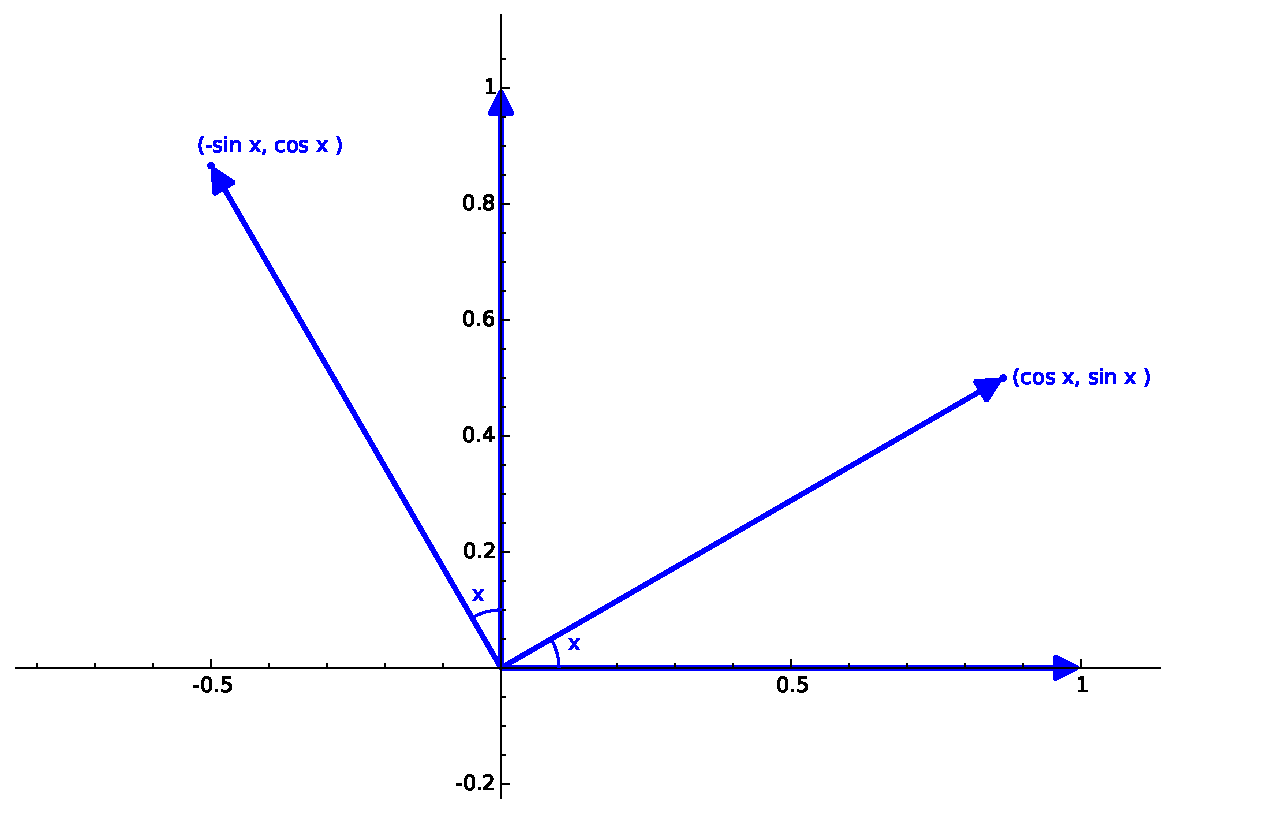
\includegraphics[scale=.75]{Rn/rotation.pdf}
\end{center}
Thus 
\begin{align*}
T(\vec{e}_1)&=\begin{bmatrix} \cos \frac{\pi}{6} \\ \sin \frac{\pi}{6}\end{bmatrix}
=\begin{bmatrix} \sqrt{3}/2 \\ 1/2\end{bmatrix}\\
T(\vec{e}_2)&=\begin{bmatrix*}[C] -\sin \frac{\pi}{6} \\ \cos \frac{\pi}{6}\end{bmatrix*}
=\begin{bmatrix*}[C] -1/2 \\ \sqrt{3}/2\end{bmatrix*}
\end{align*}
\end{example}

\subsubsection{Exercises}
\begin{exercise}
In this exerciese we are going to be deriving the standard matrix for reflection across $y=mx$. To do this we are going to rotate $y=mx$ into the $x$-axis, 
reflect across the $x$-axis, then rotate back.
\begin{enumerate}
\item Find the intersection $(x_1,y_1)$ between $y=mx$ and the unit circle $x^2+y^2=1$ that's in quadrant I or IV. Be sure to simplify any complex fractions.
\item Let $\theta=\arctan \left(\frac{y_1}{x_1}\right)$ and write the corresponding reference triangle. Use the reference triangle to compute $\cos \theta$ and $\sin \theta$ in terms of $(x_1,y_1)$.
\item Use the fact that rotation counter clockwise by $\theta$ has a standard matrix of 
$A=\begin{bmatrix*}[C]
\cos \theta & -\sin \theta \\
\sin \theta & \cos \theta \\
\end{bmatrix*}$

To find the standard matrix of rotation counter clockwise by $-\theta$. 
The transformation of this matrix will rotate $y=mx$ into the $x$-axis. Write the matrix only in terms of $(x_1,y_1)$.

\item Find the standard matrix of rotation counter clockwise by $\theta$ and write it in terms of $(x_1,y_1)$.

\item The standard matrix for reflection about the $x$-axis is $\begin{bmatrix*}[C]1 & 0 \\ 0 & -1 \end{bmatrix*}$. Mulitply these matrices to see that the 
standard matrix for reflection about $y=mx$ is 
\[
\begin{bmatrix} x_1^2-y_1^2 & 2x_1y_1 \\ 2x_1y_1 & y_1^2-x_1^2\end{bmatrix}=\frac{1}{m^2+1}\begin{bmatrix} 1-m^2 & 2m \\ 2m & m^2-1\end{bmatrix}
\]

\textbf{Note:} The matrix multiplication is a right-to-left operation. That is the operation that is first should have the matrix farthest on the right.

\end{enumerate}
\end{exercise}

\begin{exercise}
Show the standard matrix for the identity transformation 
$id:\mathbb{R}^n \to \mathbb{R}^n$ is the matrix $I=[\vec{e}_1, \vec{e}_2, \ldots, \vec{e}_n]$.
\end{exercise}

\begin{exercise} An \textbf{orthogonal matrix} is an $n \times n$ matrix with 
$A^TA=I$. Show the following standard matrices are orthogonal matrices:
\begin{enumerate}[a.)]
\item Reflection across $y=mx$
\item Rotation about $\vec{0}$ in $\mathbb{R}^2$
\item Rotation about the $x$-axis in $\mathbb{R}^3$
\item Rotation about the $y$-axis in $\mathbb{R}^3$
\item Rotation about the $z$-axis in $\mathbb{R}^3$
\end{enumerate}
\end{exercise}


\subsection{Dot Product, Distance and Angle between vectors}

\subsubsection{Exercises}

